%%%%%%
%
% PROJECT 2 - Finding the Zero of a Polynomial
%
% filename: zeros.tex
% last modified: 2014-7-22
%
%%%%%%%
%
% 
%
% 
%
%%%%%%%

\documentclass
[justified,nohyper]
{tufte-handout}

\usepackage{amsmath}
\usepackage{amsthm}


\usepackage{booktabs}
\usepackage{graphicx}
\usepackage{kmath,kerkis} % The order of the packages matters; kmath changes the default text font
\usepackage[T1]{fontenc}

\newtheoremstyle{mydef}
{\topsep}{\topsep}%
{}{}%
{\bfseries}{}
{\newline}
{%
  \rule{\textwidth}{0.4pt}\\*%
  \thmname{#1}~\thmnumber{#2}\thmnote{\ -\ #3}.\\*[-1.5ex]%
  \rule{\textwidth}{0.4pt}}%

\theoremstyle{mydef}
\newtheorem{definition}{Definition}

\begin{document}
\section{Advanced Calculus Project 2: Finding the Zero of a Polynomial}

\begin{quote}
\textbf{Instructions:} This note will not normally appear, but since this is one of your first projects, it is included here. Your first step will be to read through the entire project description below to get a feel for what this project is about and what work you will need to do. One of the first steps will be for you to get the essence of the project inside your head and begin to think about it. For this project, we will be doing a lot with equations of tangent lines, finding the zero of a polynomial, and extending the ideas to include quadratic tangents.

In this report, there are several guiding questions and specific steps you are asked to do. One of the things you will need to do in your writeup is to gather all these suggestions together and develop your own flow for the report. By this, I mean that you should not simply answer the questions I ask in the project description. You will need to decide on an abstract for the report that incorporates the ideas described in this project description. You will need to decide on some sort of conclusion based on the work done. Most importantly, your writeup should stand alone. By this, I mean that anyone with a reasonable background in Calculus could pick up a copy of your report and read it without having to refer back to this project description. I imagine that this may take some practice since this is the first time you've been asked to do something like this. Based on feedback from me, you may need to re-write your first couple of projects. If this happens, it is perfectly ok. You will improve and your reports will improve.
\end{quote}

\newthought{Consider the polynomial} $P(x)=x^3+3x-1$. Your goal is to find a zero of this function: i.e., a number $a$ such that $P(a)=0$. Although there is an algebraic technique for finding a zero of a cubic polynomial, we are going to approximate a zero. We want the approximation to be within $10^{-2}$ of an actual zero.

In this project, you will approach this problem using three different techniques. The first technique will use a method of bisection. The second will use a tangent line. The third will use a tangent quadratic. The conclusion of your report must compare and comment on these three ways of solving the same problem.

To begin, show that the equation $P(x)=0$ has at least one solution in the interval $[-1,1]$. You must give a good justification that such a solution exists.

The bisection method to approximate a zero of $P(x)$ starts with the interval $[-1,1]$. Bisecting this interval into two pieces means that you split $[-1,1]$ into $[-1,0]$ and $[0,1]$. Determine whether $P(x)=0$ has a solution in $[-1,0]$ or $[0,1]$ (as you did with the original interval $[-1,1]$), and then repeat the process of bisection with the new interval containing a solution. How many times must you repeat the bisection process to have a sufficiently accurate answer? Find such an answer.

\newpage

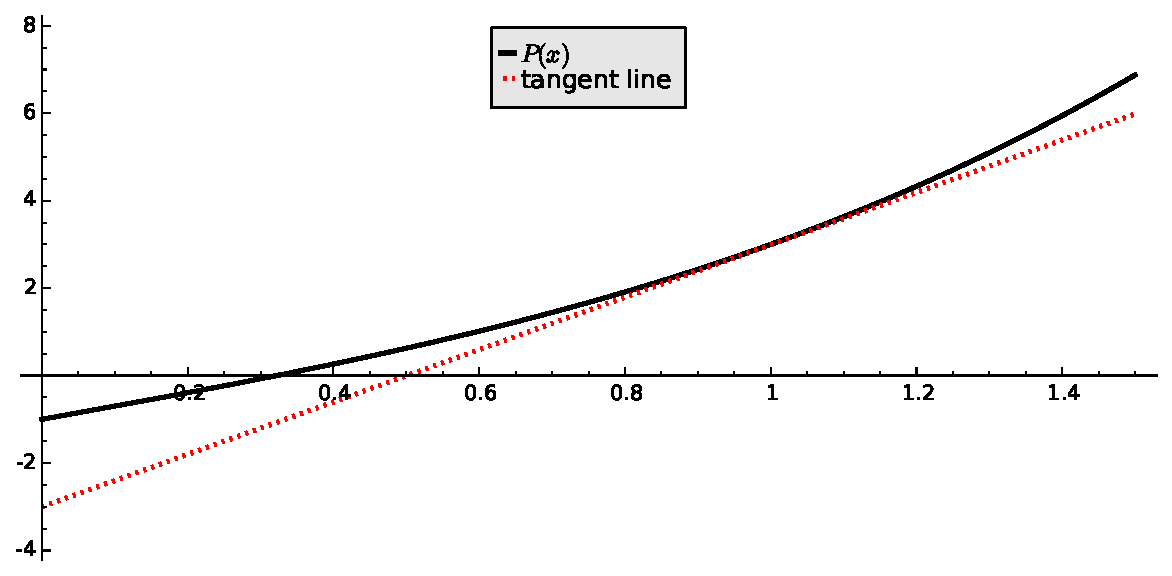
\includegraphics[width=10cm]{p_of_x.pdf}

Calculus gives us another way to perform the search for a zero of $P(x)$. In the figure shown above, I have graphed $P(x)$ and the tangent to $P$ when $x=1$. We will use the idea that the tangent line is a good approximation to the graph of a function (also known as local linearity). Suppose that $a$ is some $x$-value and we want to find the equation of the tangent line to $P$ at $x=a$. What is the $x$-intercept of this tangent line in terms of $a$, $P(a)$, and $P'(a)$? Draw a picture to demonstrate what is going on.

Using this expression for the $x$-intercept, let's try and find a zero of $P(x)$. Begin with one of the end points of the original interval; this is your original guess for a zero of $P(x)$ (i.e. the value of $a$ will be either $-1$ or $1$). Find the $x$-intercept of the tangent line as a new guess, which hopefully is a better approximation to a solution of the equation $x^3+3x-1=0$ than the end point you started with. It should be evident from the graph shown above that the $x$-intercept of the tangent line is closer to the zero of $P(x)$ than the original guess of $x=1$. Is this $x$-intercept within the desired margin of error from the answer you obtained using the method of bisection? If not, use the $x$-intercept as the value of $a$ and find a new tangent line to $P$. Find the $x$-intercept of this new tangent line and see if it is a closer approximation to a zero of $P$. Repeat this process until you have found a zero to within the desired degree of accuracy.

Compare the two techniques (bisection versus tangent line) for finding a solution. Which is easier to understand? Why? Which is faster -- that is, which leads to an answer within the desired degree of accuracy in the fewest number of iterations?

Instead of using a tangent line, we could use a ``tangent quadratic.'' For any curve given by $g(x)$, it would seem that a quadratic function could do a better job of staying close to $g$ than a straight line. If that's the case, would it make sense that we could use a tangent quadratic instead of a tangent line to approximate a zero of a function?

When you construct a tangent line to a function at a point, you needed two things: the slope of the curve at that point and the coordinates of the point on the curve. The tangent line has the same slope as the curve at that point. For a tangent quadratic, start with a general quadratic $q(x)=ax^2+bx+c$ and think about how to determine the constants $a$, $b$, and $c$ so that $q(x)$ has the appropriate properties.

In your report, you should clearly define how to find a tangent quadratic. Also, would a tangent quadratic work in place of the tangent line for approximating a zero of a function? What problems would arise? How do you think it would compare to the two techniques above? Try out the new tangent quadratic using the given $P(x)$ by approximating the zero in the interval given.

Your graphing calculator (Ti-84 or equivalent) has a zero-finding capability. If you enter the polynomial $P(x)$ for $Y1$, look at the graph, press 2$^{nd}$-calc, select ZERO, and enter left and right bounds, the calculator will locate the zero. Why do you suppose it is important for the calculator to have left and right bounds? Will any left and right bound work? How are these bounds related to the original interval of $[-1,1]$ in this project? You may want to spend a little time experimenting with your calculator to see if you can discover how to make it fail to find a zero. As part of your final report, you should comment on the importance of these bounds and what they do in the context of finding the zero of a function.

\end{document}
%sagemathcloud={"zoom_width":125}
